\chapter{Sviluppo dei contenuti}

\section{Attività 1: Introduzione alla ricorsione}

\clm{}{}{Bisogna inzialmente introdurre in linea generale il contenuto
dell'attività agli studenti, facendo attenzione a non perdersi nei dettagli
che verranno approfonditi durante le fasi successive. Questo 
aiuta ad accendere la curiosità degli studenti e a farli partecipare
attivamente all'attività.
}

\nt{In questo documento ho inserito note specifiche per gli insegnanti
(come quella sopra). Tuttavia sono solo brevi suggerimenti, in quanto
la guida per gli insegnanti vera e propria è contenuta nella sezione
seguente. }

\paragraph{Materiale utilizzato in questa fase:}

\begin{itemize}
    \item [$\Rightarrow$] Lavagna multimediale;
    \item [$\Rightarrow$] Computers.
\end{itemize}

\clm{}{}{In questa fase i computers sono opzionali. Il docente può, a discrezione personale,
decidere di condividere sui computers degli studenti il codice di esempio (per una maggiore interazione)
oppure mostrarlo sulla lavagna multimediale.}

\paragraph{Fase 1:}

\begin{itemize}
    \item [$\Rightarrow$] \textbf{\textcolor{cyan}{Consegna:}} come prima cosa, per introdurre
    quest'attività si consiglia di ripassare brevemente i tipi di dati (Int, float, etc.). 
    Successivamente il docente introduce la ricorsione spiegando i concetti di passo base e passo
    ricorsivo. Per supportare quest'attività si può fare riferimento al primo esercizio di programmazione proposto
    (Fibonacci ricorsivo). Al termine di questa fase si dovranno anche introdurre gli elementi sintattici basilari di Haskell.
    \item [$\Rightarrow$] \textbf{\textcolor{magenta}{Svolgimento:}} inizialmente si presenterà la
    ricorsione in maniera discorsiva anche facendo esempi legati alla quotidianetà 
    (per esempio un \texttt{\href{https://www.researchgate.net/publication/309578166_Percorso_didattico_sulla_ricorsione_dalla_natura_al_coding}{treno}}:
    se ha 1 solo vagone, passo base, allora è semplicemente un vagone. Se ha n > 1 vagoni allora
    è un treno composto da una "testa" e da n - 1 vagoni). Eventualmente si possono anche mostrare,
    su una lavagna multimediale, immagini che presentano la ricorsione (per esempio alcuni dei quadri di Escher
    come "Mani che disegnano" o "Cascata"). Dopo di ché gli studenti verranno incoraggiati a partecipare portando
    ulteriori esempi di ricorsività sulla base delle loro esperienze personali.
     Infine si mostra l'esempio riguardante Fibonacci, scritto in Haskell
    e si approfittà per dare un'idea concreta di utilizzo di ricorsione.
    \item [$\Rightarrow$] \textbf{\textcolor{teal}{Discussione:}} il docente dovrà gestire una discussione
    sulla base degli esempi portati dagli studenti e correggere eventuali errori concettuali
    tramite il dialogo. 
    \item [$\Rightarrow$] \textbf{\textcolor{orange}{Conclusione:}} Per concludere quest'attività il docente introdurrà
    la sintassi base di Haskell (insieme all'utilizzo di GHCI) e si assicurerà che essa venga compresa dagli studenti. 
\end{itemize}

\clm{}{}{Può essere utile, prima di proseguire con l'attività unplugged, porre alcune 
domande agli/alle studenti/studentesse per assicurarsi che abbiano compreso le basi su cui si sviluppa la ricorsione.
Si può prendere spunto dalla sezione riguardante gli "Indicatori" presente nel capitolo successivo.}

\nt{Comandi utili di GHCI:
\begin{itemize}
    \item \texttt{:load} o \texttt{:l}, serve per compilare un file hs (Haskell);
    \item \texttt{:type} o \texttt{:t}, mostra il tipo di una funzione;
    \item \texttt{:reload} o \texttt{:r}, ricompila tutti i file precedentemente compilati;
    \item \texttt{:!clear}, pulisce lo schermo del terminale di GHCI (solo linux).
\end{itemize}
}

\section{Attività 2: Le Matrioske (unplugged)}\label{unplugged}

\paragraph{Materiale utilizzato in questa fase:}

\begin{itemize}
    \item [$\Rightarrow$] Matrioske;
    \item [$\Rightarrow$] Adesivi;
    \item [$\Rightarrow$] Fogli di carta;
    \item [$\Rightarrow$] Penne.
\end{itemize}

\clm{}{}{
\begin{itemize}
    \item In alternativa agli adesivi si possono usare cartoncini e nastro adesivo;
    \item Se non ci sono abbastanza matrioske per tutti si possono formare dei gruppetti;
    \item Il valore che viene utilizzato non è importante, si è scelto di utilizzare "1" 
    a titolo indicativo;
    \item Se si decide di usare un numero diverso da "1" si deve tenere presente che i passi
    ricorsivi, ossia le matrioske non più interne, devono avere tutte lo stesso valore.
\end{itemize}    
}

\paragraph{Fase 1:}

\begin{itemize}
    \item [$\Rightarrow$] \textbf{\textcolor{cyan}{Consegna:}} si utilizzano le matrioske per spiegare 
    il concetto di funzione ricorsiva. Come fase preliminare, il docente deve aver attaccato a ogni matrioska 
    un adesivo con scritto "Aprimi e aggiungi 1 al valore al mio interno", con l'eccezione delle matrioske più interno che avranno
    un adesivo con la scritta "1".
    \item [$\Rightarrow$] \textbf{\textcolor{magenta}{Svolgimento:}}
    \begin{enumerate}
        \item Viene fornita una matrioska (prepata precedentemente dal docente secondo la consegna) a ciascun studente/studentessa (o gruppo di studenti);
        \item Vengono fornite penne e fogli di carta a ogni studente/studentessa;
        \item Ogni studente/studentessa legge l'adesivo attaccato alla matrioska e ne riporta la scritta
        su un foglio;
        \item Ogni studente/studentessa apre, se possibile\footnote{La matrioska non ha attaccato l'adesivo con la scritta "1".},
        la matrioska;
        \item Si ripetono i punti 3 e 4 finché possibile. Se non è possibile si passa al punto 6;
        \item Ogni studente/studentessa esegue le istruzioni che ha trascritto sul foglio cominciando dalla penultima (in quanto l'ultima e semplicemente "1")
        e proseguendo a ritroso.
    \end{enumerate}
    \item [$\Rightarrow$] \textbf{\textcolor{teal}{Discussione:}} Il docente comincia la discussione chiedendo agli/alle alunni/e 
    che valore è risultato seguendo questo processo. Successivamente si possono portare
    gli/le studenti/studentesse a ragionare su cosa sia questo valore (nel caso dell'esempio proposto con "1" 
    il risultato rappresenta il numero di matrioske di cui è composta la matrioska). Per concludere il dibattito
    si fa notare che, in questo caso, il risultato si comporta come una variabile "contatore" che aumenta di "1"
    per ogni matrioska. Questo serve per creare un collegamento cognitivo con il concetto più familiare di
    iterazione, ma allo stesso tempo mostra che ci sono modi alternativi di vedere un problema.  
    \item [$\Rightarrow$] \textbf{\textcolor{orange}{Conclusione:}} Il docente si assicura che ogni
    alunno/a abbia capito cosa è stato fatto in questa fase e quali siano le implicazioni di ciò. 
\end{itemize}

\subsection{Da Unplugged a Programmazione (Fase 2 de "Le Matrioske")}

\paragraph{Materiale utilizzato in questa fase:}

\begin{itemize}
    \item [$\Rightarrow$] Fogli di carta;
    \item [$\Rightarrow$] Penne;
    \item [$\Rightarrow$] Lavagna multimediale;
    \item [$\Rightarrow$] Computers.
\end{itemize}

\clm{}{}{Non ci si deve soffermare sugli aspetti tecnici del codice in quanto molto
avanza (do, let, show, monade IO()), ma ci si concentra sulla funzione per costruire le matrioske.

La funzione \texttt{costruisciMatrioska} riceve in input un numero corrispondente a quante matrioske si vuole racchiudere
e restituisce la matrioska corrispondente (ogni matrioska è indicata da un livello numerico).
}


\paragraph{Fase 2:}

\begin{itemize}
    \item [$\Rightarrow$] \textbf{\textcolor{cyan}{Consegna:}} Si continua a ragionare sulle matrioske
    e sulla ricorsione utilizzando il codice lasciato in calce a questa sezione. Il codice può
    essere mostrato sulla lavagna multimediale oppure essere condiviso con gli/le studenti/studentessa in
    modo che possano vederlo sul proprio computer.
    \item [$\Rightarrow$] \textbf{\textcolor{magenta}{Svolgimento:}}
    \begin{enumerate}
        \item Mostrare e/o condividere il codice al fondo della sezione con gli/le studenti/studentesse;
        \item L'insegnante spiega brevemente che cosa fa la funzione \texttt{costruisciMatrioska};
        \item Ogni studente/studentessa scrive su un foglio (ricevuto nella fase precedente) un ipotesi
        sull'output del programma mostrato;
        \item A turno, chi vuole, può provare a illustrare alla classe il risultato a cui si è arrivati spiegando i ragionamenti fatti;
        \item Si possono ripetere a piacere i precedenti due passaggi variando l'intero passato come parametro
        alla funzione \texttt{costruisciMatrioska}.
    \end{enumerate}
    \item [$\Rightarrow$] \textbf{\textcolor{teal}{Discussione:}} Si può far ragionare su come la rappresentazione
    di una matrioska sia resa in maniera molto elegante dall'utilizzo della ricorsione e che, utilizzando cicli (programmazione interativa),
    non si riuscirebbe a dare efficacemente l'idea di "matrioska annidata dentro un'altra matrioska" che,
    viene fornita intuitivamente dal codice Haskell mostrato. 
    \item [$\Rightarrow$] \textbf{\textcolor{orange}{Conclusione:}} L'insegnante si assicura
    che tutti abbiano prestato attenzione all'esercizio e riassume brevemente i punti fondamentali
    di questa fase soffermandosi sull'alta leggibilità di una soluzione ricorsiva e sulla sua utilità.
\end{itemize}

\paragraph{Semplice analisi del codice:}

\begin{itemize}
    \item \texttt{data Matrioska...}: rappresenta la dichiarazione di una struttura dati chiamata
    Matrioska. Questa struttura dati è ricorsiva ed è formata da una "M", una stringa e una lista di Matrioske (per questo è ricorsiva).
    L'ultima parte (\texttt{deriving show}) serve unicamente per la stampa;
    \item \texttt{costruisciMatrioska :: Int -> Matrioska:} è la funzione più importante per quest'attività.
    Prende in input un intero "n" e restituisce una Matrioska a "n" livelli, ossia composta da "n" matrioske.
    Per fare ciò se l'intero "n" è diversoda 0 o da 1 chiama ricorsivamente sé stessa passando l'intero "n" meno 1;
    \item \texttt{stampareMatrioske :: Matrioska -> IO():} utilizzando la monade IO(), e la sintassi avanzata di Haskell, 
    stampa una Matrioska;
    \item \texttt{main :: IO():} il main del programma. Si occupa di costruire una Matrioska a 5 livelli (può essere cambiato a piacimento)
    e di stampare la Matrioska così creata.
\end{itemize}

\begin{figure}[!h]
    \centering
    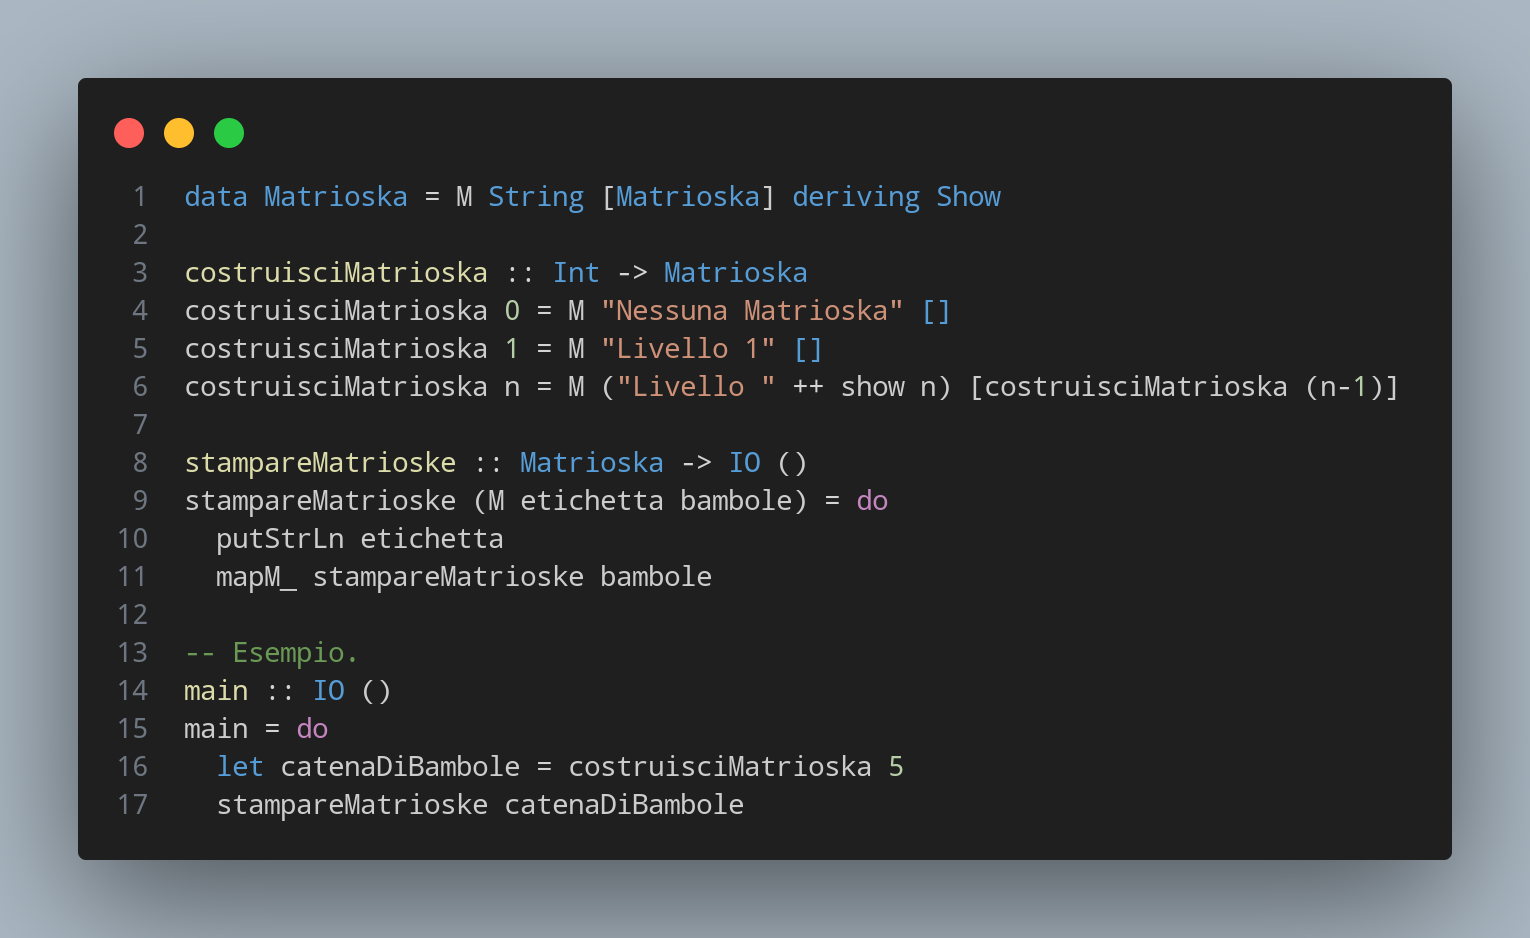
\includegraphics[width=1\textwidth]{images/Matrioske.png}
\end{figure}

\clearpage

\section{Attività 3: Programmazione in Haskell}

\paragraph{Materiale utilizzato in questa fase:}

\begin{itemize}
    \item [$\Rightarrow$] Lavagna multimediale;
    \item [$\Rightarrow$] Computers.
\end{itemize}

\clm{}{}{Per ora gli esercizi con la scritta "Parte avanzata" non sono necessari, in quanto possibile estensione
dell'attività.}

\paragraph{Fase 1:}

\begin{itemize}
    \item [$\Rightarrow$] \textbf{\textcolor{cyan}{Consegna:}} Ripassare brevemente i concetti base di Haskell. Successivamente
    si andranno a eseguire, individualmente o a coppie (a discrezione dell'insegnante), una serie di esercizi mirati su Haskell. 
    \item [$\Rightarrow$] \textbf{\textcolor{magenta}{Svolgimento:}}
    \begin{enumerate}
        \item Il docente introduce brevemente le liste, gli operatori e le principali funzioni su di esse;
        \item Il docente assegna un esercizio per tipologia ("per prendere confidenza", "sulle guardie", "sulle liste", "sulla ricorsione esplicita");
        \item Gli/Le studenti/studentesse svolgeranno, individualmente o in coppia, gli esercizi proposti;
        \item Ogni studente/studentessa illustra le sue soluzioni alla classe giustificando le proprie implementazioni.
    \end{enumerate}
    \item [$\Rightarrow$] \textbf{\textcolor{teal}{Discussione:}} Si discutono le soluzioni avanzate dagli/dalle studenti/studentesse.
    L'insegnante ha il compito di mediare il dialogo e suggerire implementazioni altenative mostrando come, all'interno dell'ambito della ricorsione,
    ci siano modi differenti di vedere un problema.
    \item [$\Rightarrow$] \textbf{\textcolor{orange}{Conclusione:}}  
\end{itemize}

\pagebreak

\section{Esercizi di programmazione}\label{prog}

\subsection{Esempio}

\paragraph{Fibonacci ricorsivo:} viene usato nella prima parte dell'attività come esempio
di utilizzo della ricorsione.

\begin{figure}[!h]
    \centering
    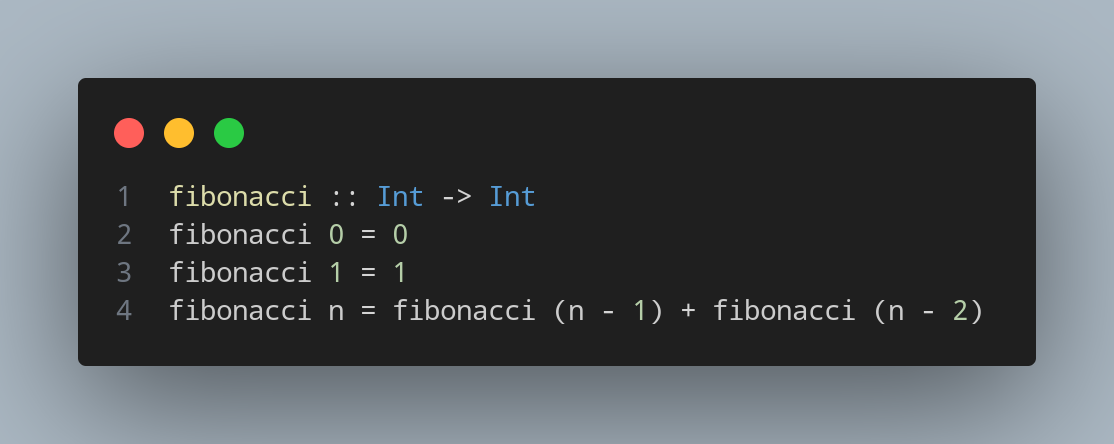
\includegraphics[width=0.5\textwidth]{images/Fibonacci.png}
\end{figure}

\subsection{Esercizi per prendere confidenza}

\paragraph{Somma:} Scrivere una funzione in Haskell (con tipo \texttt{Int -> Int}), 
che prenda in input un intero n e calcoli la somma dei primi n numeri naturali.

\begin{figure}[!h]
    \centering
    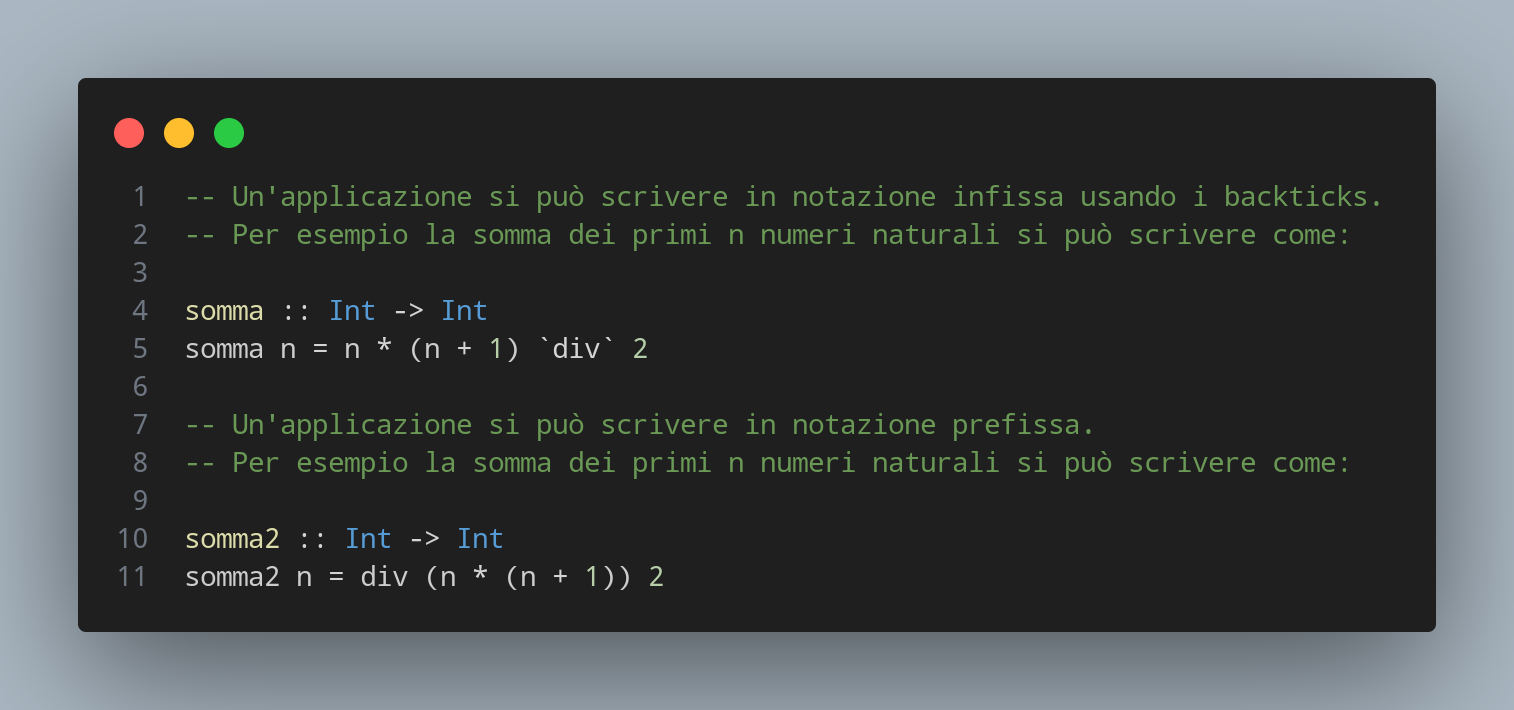
\includegraphics[width=0.8\textwidth]{images/Somma.png}
\end{figure}

\paragraph{Area:} Scrivere una funzione in Haskell (con tipo \texttt{Float -> Float}), 
che calcoli l'area di un cerchio prendendo in input il suo raggio.

\begin{figure}[!h]
    \centering
    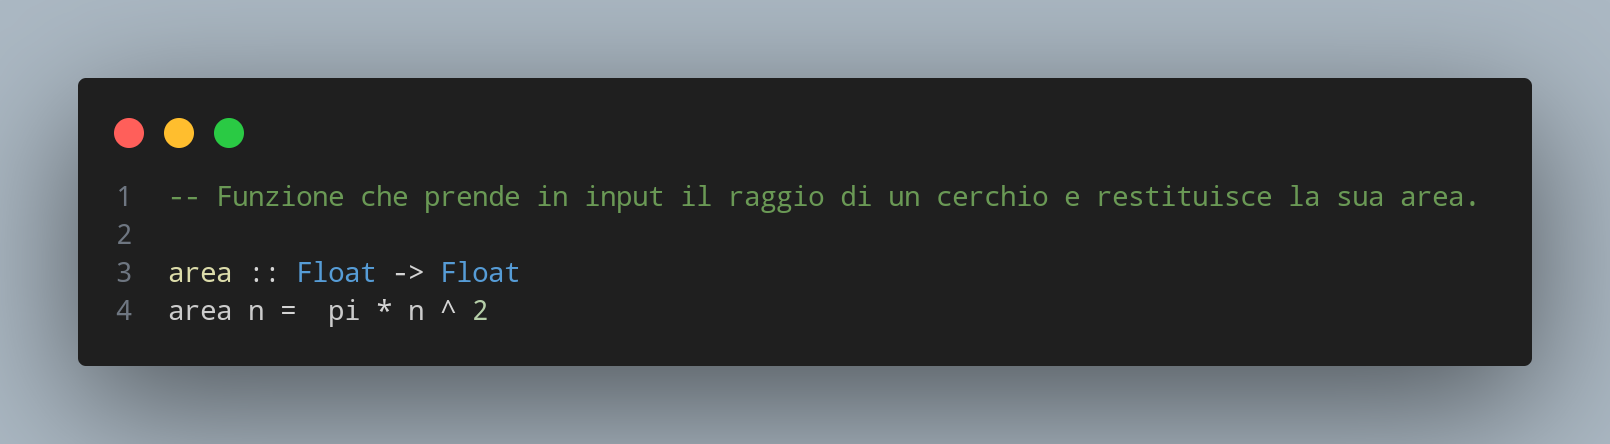
\includegraphics[width=0.8\textwidth]{images/Area.png}
\end{figure}
\pagebreak
\subsection{Esercizi sulle guardie}

\paragraph{Massimo:} Scrivere una funzione in Haskell (con tipo \texttt{Int -> Int -> Int}), usando 
le guardie, che
prenda in input due interi e restituisca il maggiore.

\begin{figure}[!h]
    \centering
    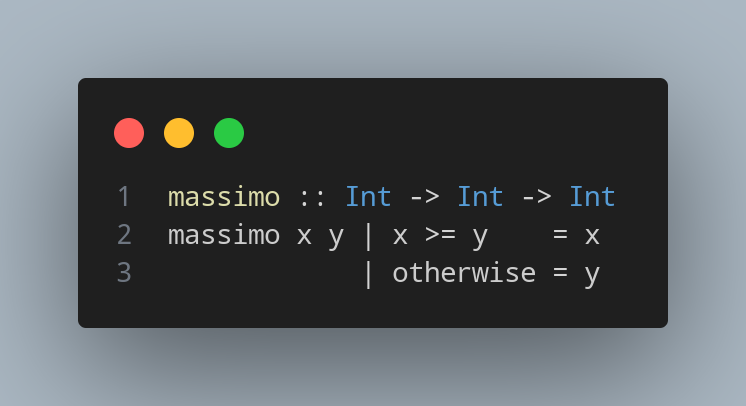
\includegraphics[width=0.5\textwidth]{images/Massimo.png}
\end{figure}

\paragraph{Massimo:} Scrivere una funzione in Haskell (con tipo \texttt{Int -> Int -> Int}), usando 
le guardie, che
prenda in input due interi e restituisca il minore.

\begin{figure}[!h]
    \centering
    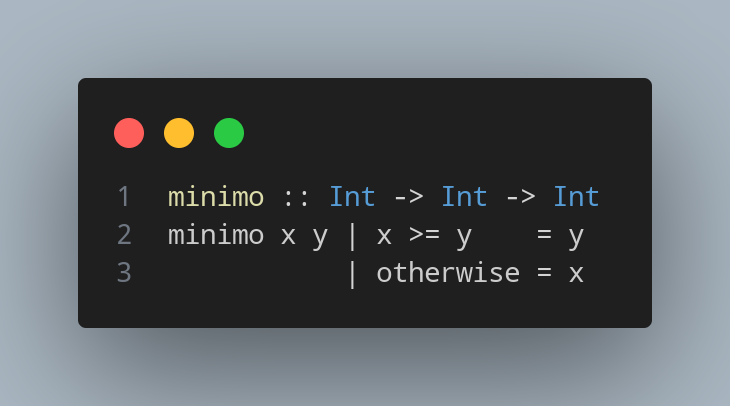
\includegraphics[width=0.5\textwidth]{images/Minimo.png}
\end{figure}

\pagebreak

\subsection{Esercizi sulle liste}

Prima di iniziare gli esercizi con le liste si deve condividere questa "dispensa"
che illustra le principali caratteristiche delle liste.

\begin{figure}[!h]
    \centering
    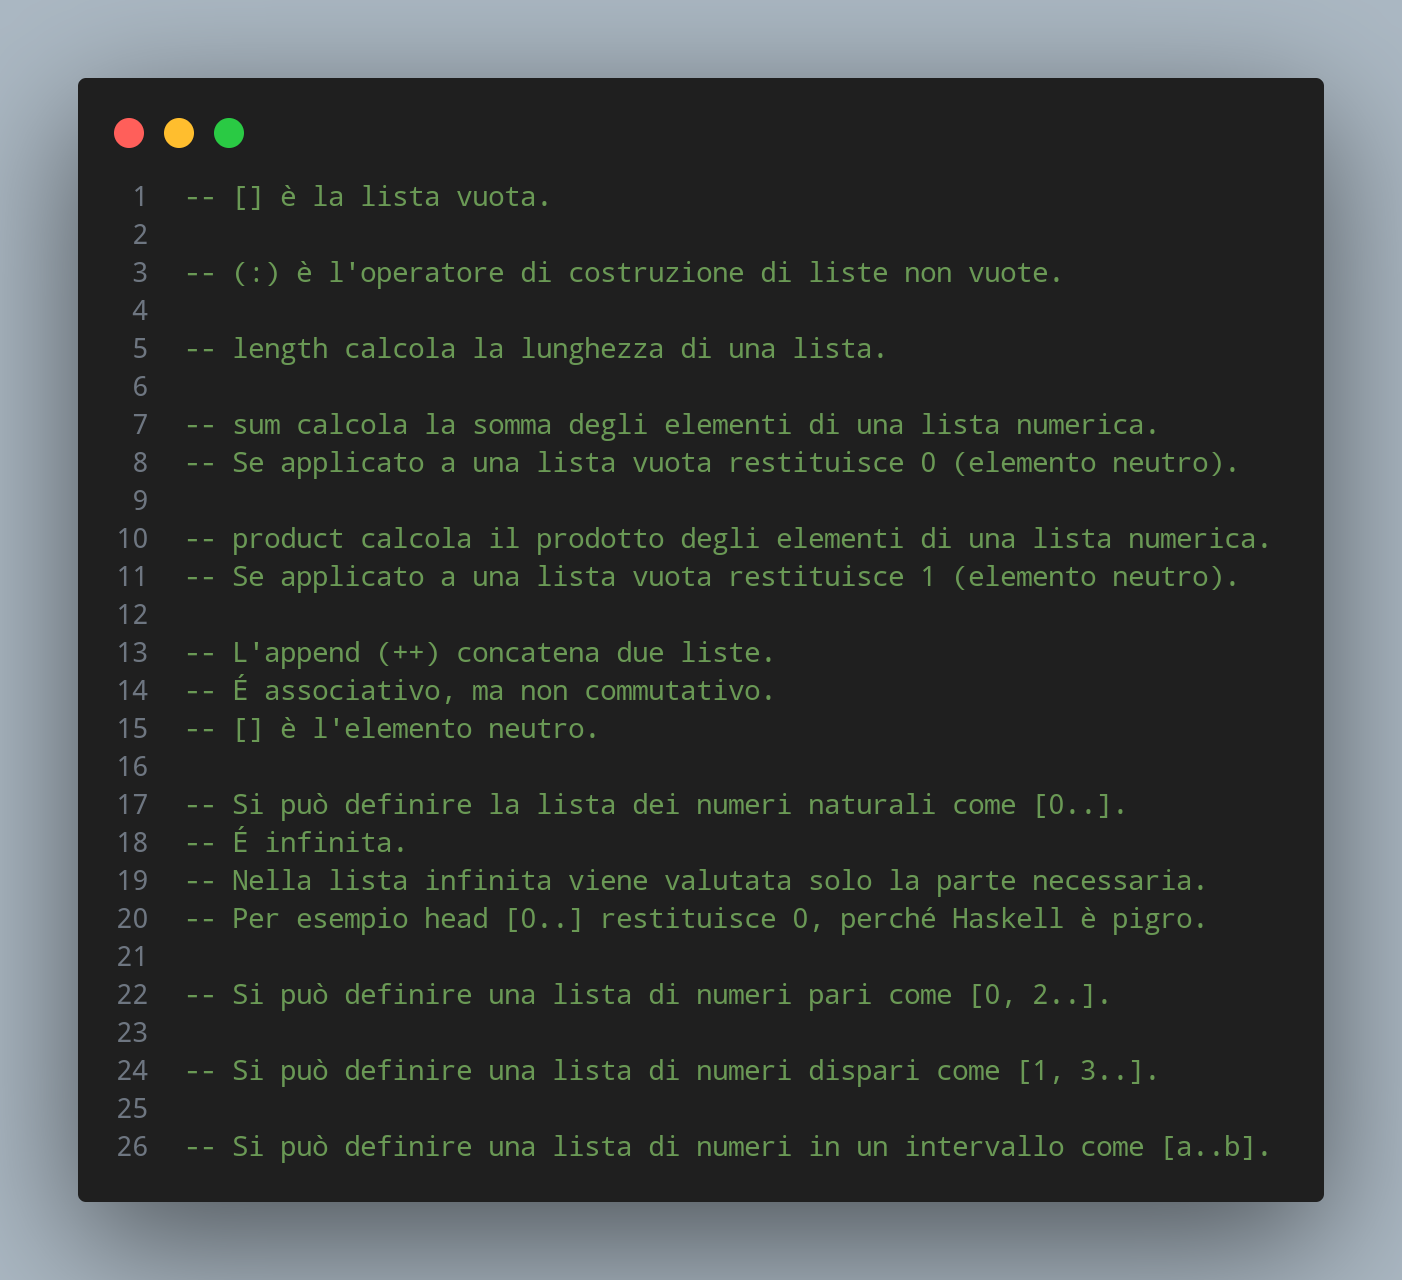
\includegraphics[width=1\textwidth]{images/Dispensa liste.png}
\end{figure}

\pagebreak

\paragraph{Fattoriale:} Scrivere una funzione in Haskell (con tipo \texttt{Int -> Int}), usando 
le liste, che prende in input un intero e restituisca il fattoriale di quel numero.

\clm{}{}{Se gli/le studenti/studentesse si trovano in difficoltà si può suggerire loro
di far uso della funzione di libreria \texttt{product} vista precedentemente.}

\begin{figure}[!h]
    \centering
    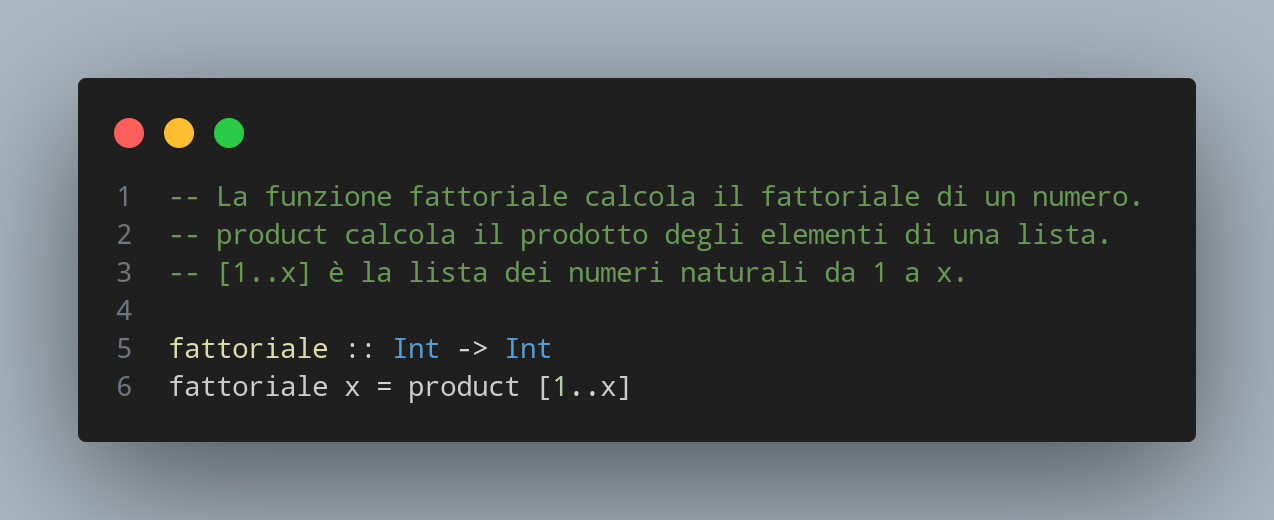
\includegraphics[width=0.7\textwidth]{images/Fattoriale.png}
\end{figure}

\paragraph{Intervallo:} Scrivere una funzione in Haskell (con tipo \texttt{Int -> Int -> [Int]}), 
che dati in input due interi calcoli la lista di interi compresi tra quei due numeri. Suggerimento:
usare la ricorsione.

\begin{figure}[!h]
    \centering
    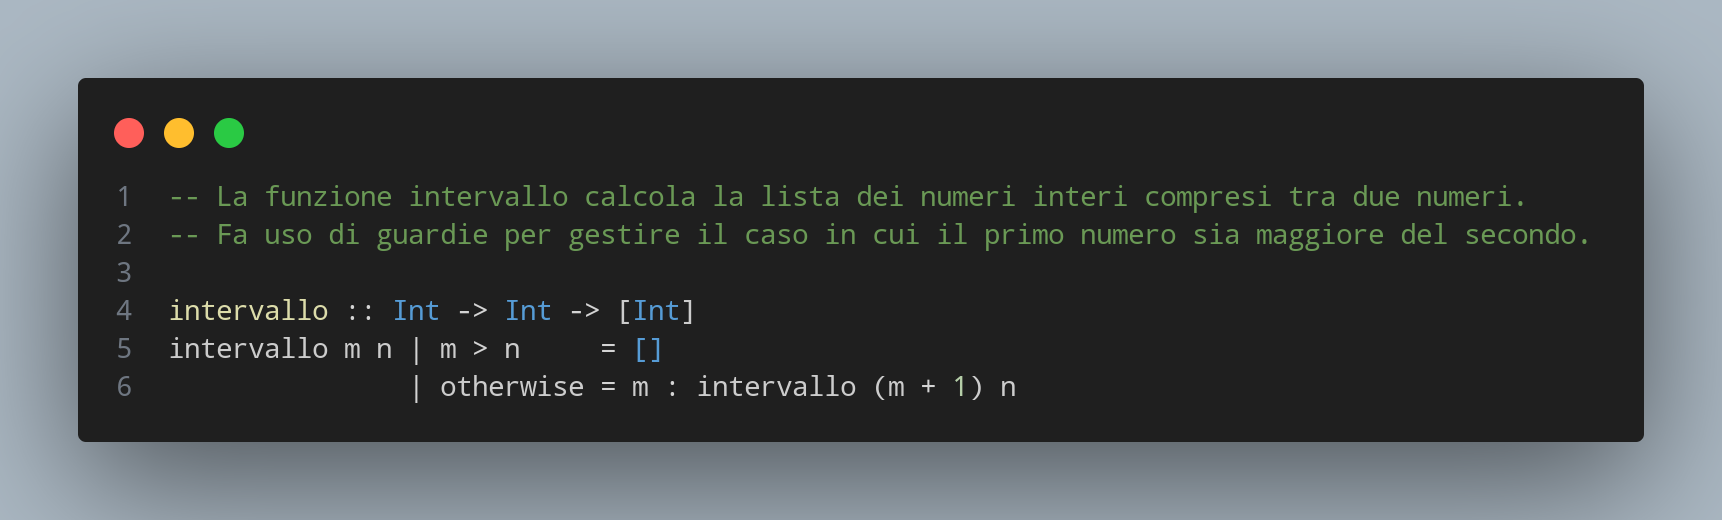
\includegraphics[width=0.8\textwidth]{images/Intervallo.png}
\end{figure}
\pagebreak
\subsection{Esercizi sulla ricorsione esplicita}

\paragraph{Somma ricorsiva:} Scrivere una funzione in Haskell (con tipo \texttt{Int -> Int}), 
che prenda in input un intero n e calcoli la somma dei primi n numeri naturali, utilizzando la ricorsione.

\begin{figure}[!h]
    \centering
    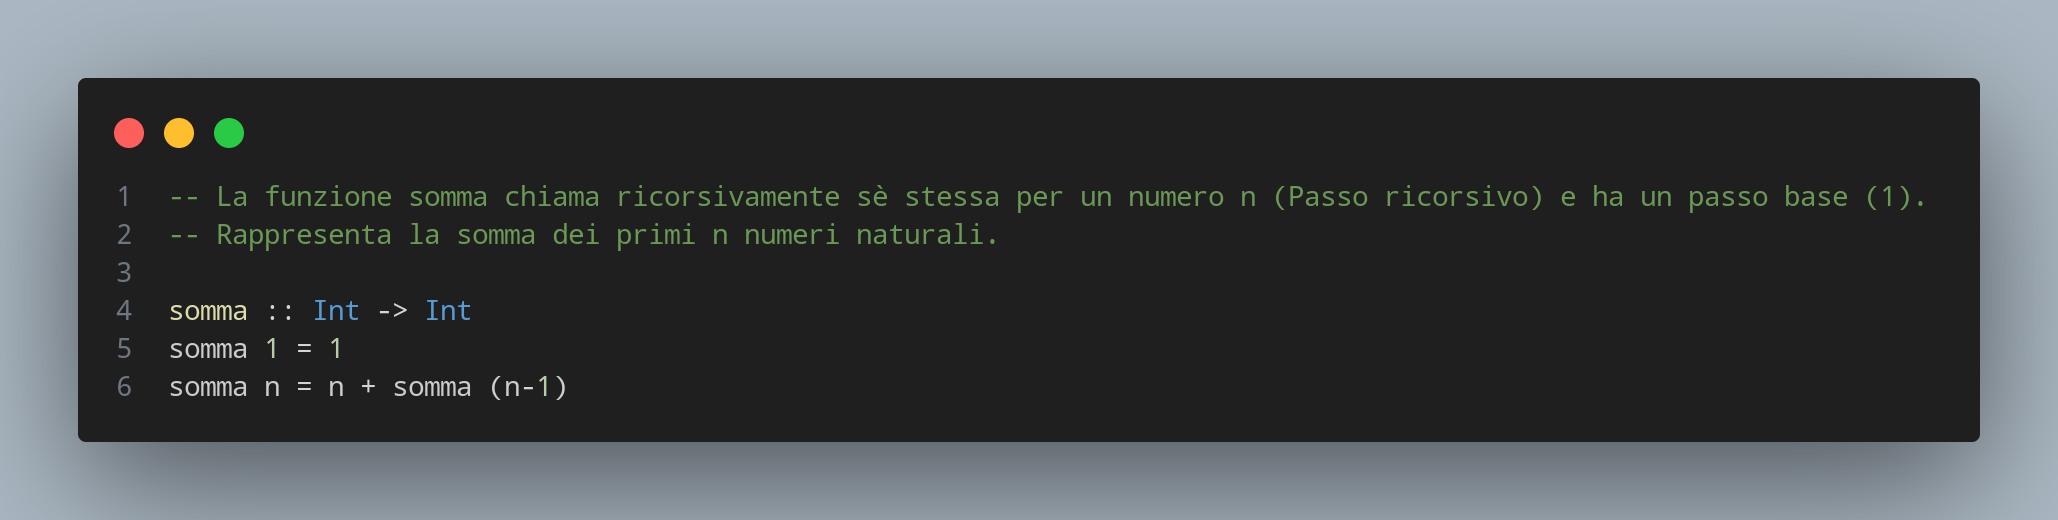
\includegraphics[width=1\textwidth]{images/Somma2.png}
\end{figure}

\paragraph{Fattoriale ricorsivo:} Scrivere una funzione in Haskell (con tipo \texttt{Int -> Int}),
che prende in input un intero e restituisca il fattoriale di quel numero, usando la ricorsione.

\begin{figure}[!h]
    \centering
    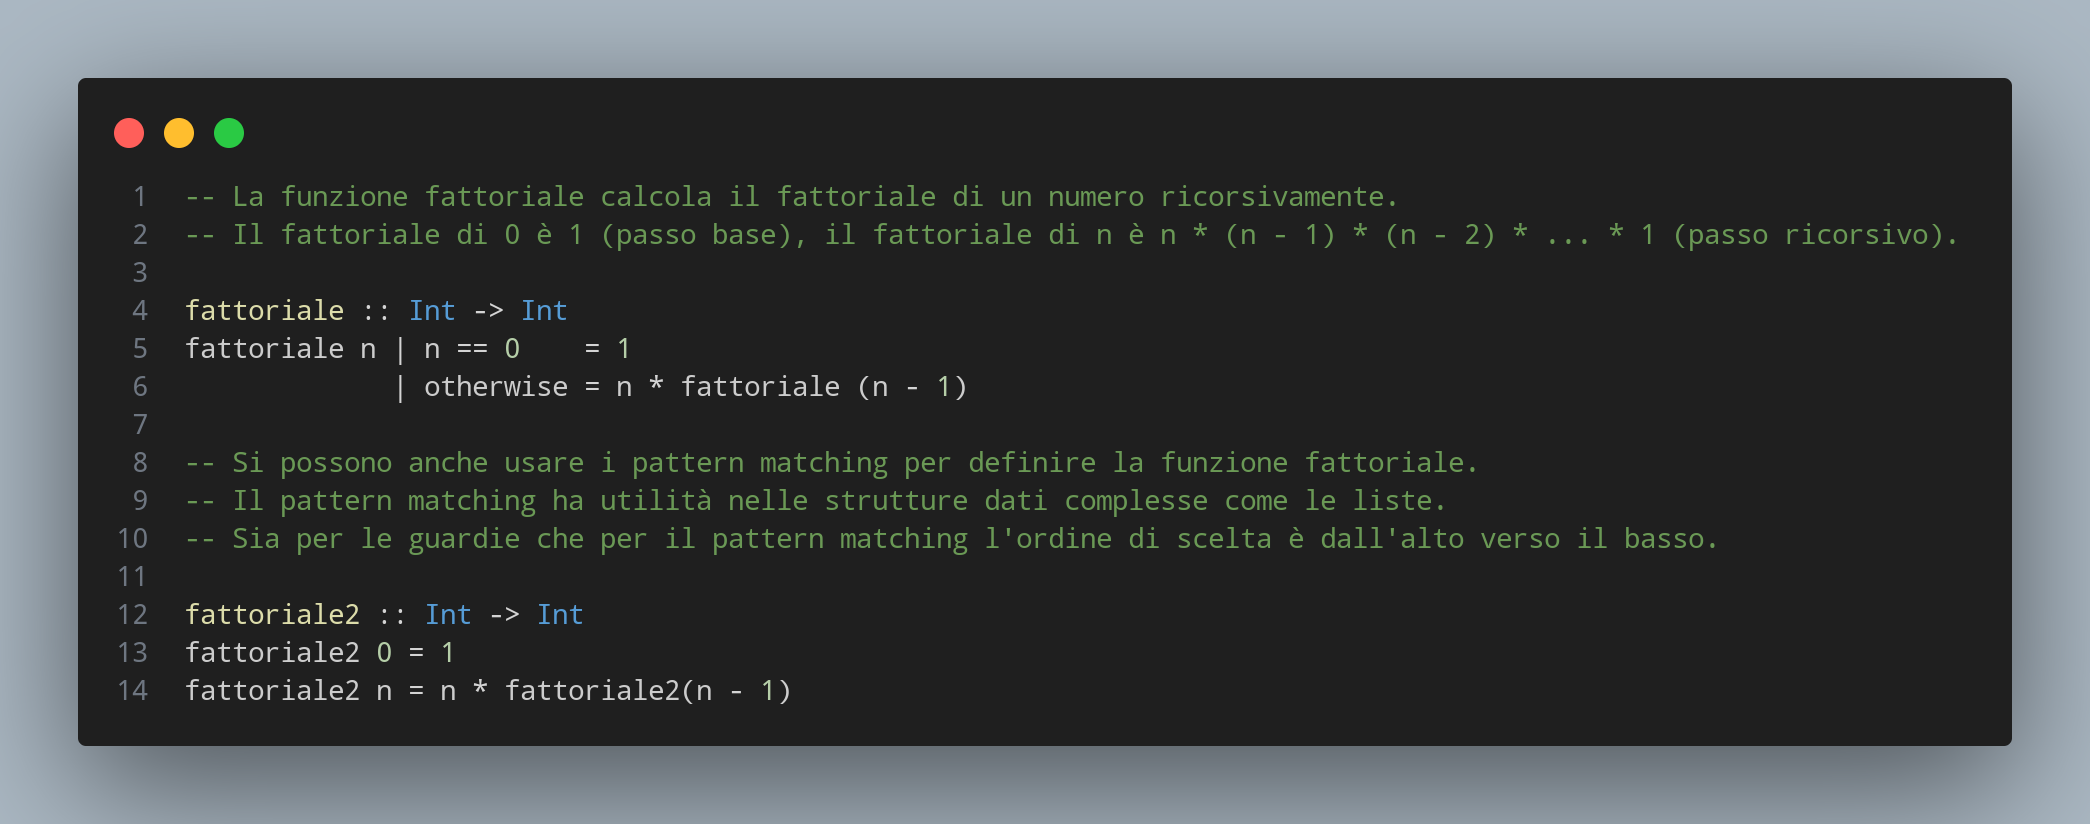
\includegraphics[width=1\textwidth]{images/Fattoriale2.png}
\end{figure}

\paragraph{Potenze di 2:} Scrivere una funzione in Haskell (con tipo \texttt{Int -> Int}),
che prende in input un intero e restituisca 2 elevato a quell'intero, usando la ricorsione.

\begin{figure}[!h]
    \centering
    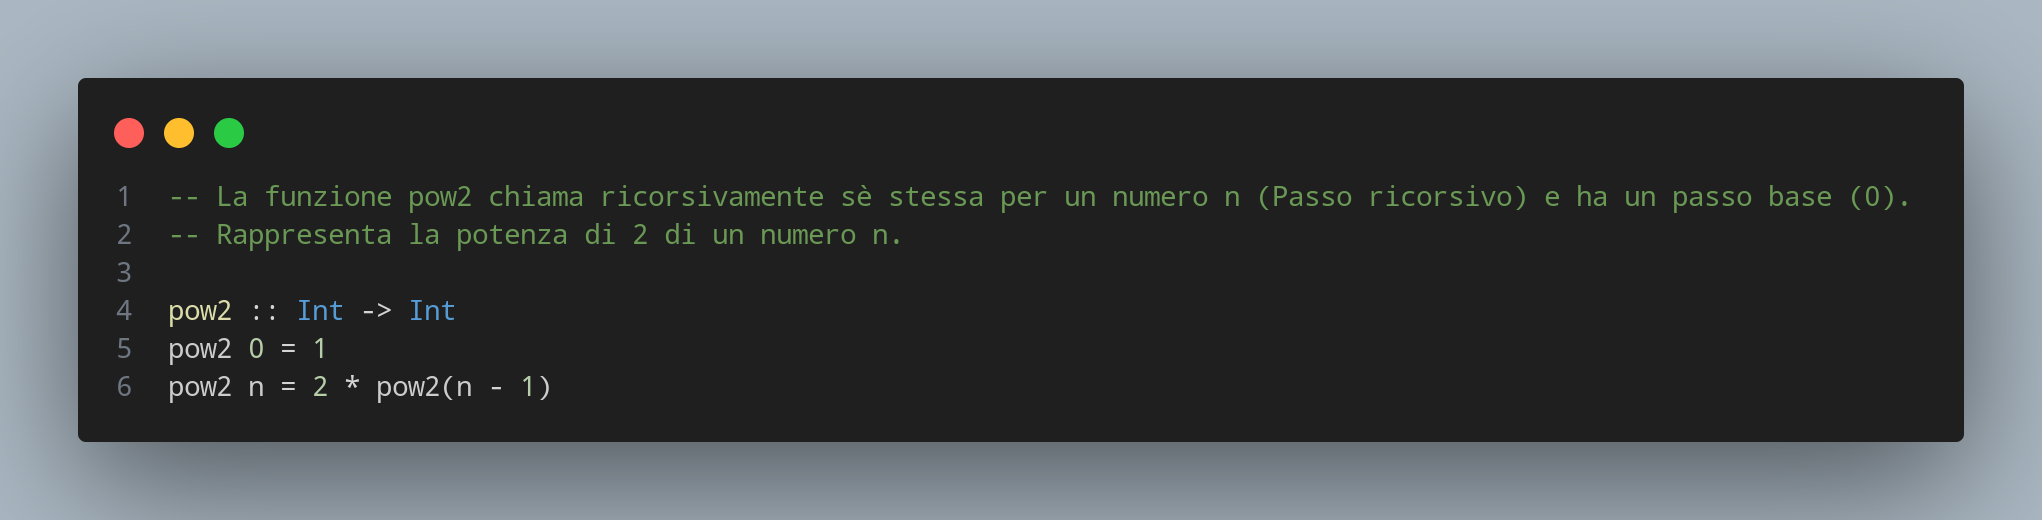
\includegraphics[width=1\textwidth]{images/Pow2.png}
\end{figure}

\pagebreak

\subsection{Parte avanzata: esercizi sugli alberi}